\documentclass[12pt, letterpaper]{article}
\usepackage[utf8]{inputenc}
\usepackage[spanish,es-noquoting]{babel}
\usepackage{amsmath, amssymb, amsthm, bm}
\usepackage{graphicx}
\usepackage{array}
\usepackage{hyperref}
\usepackage{enumitem}
\usepackage{float}
\usepackage{xcolor}
\usepackage{booktabs}
\usepackage{tikz}
\usetikzlibrary{automata, positioning, arrows.meta}
\definecolor{lightgray}{rgb}{0.95,0.95,0.95}
%% Sets page size and margins
\usepackage[top=2.5cm,bottom=2.5cm,left=2cm,right=2cm]{geometry}
\usepackage{setspace}
\onehalfspacing
\usepackage{gensymb}
\usepackage{fancyhdr}
\pagestyle{fancy}
\fancyhead[L]{Compiladores}
\fancyhead[C]{Tarea 2}
\fancyhead[R]{Facultad de Ciencias UNAM}
\fancyfoot[C]{\thepage}
\renewcommand{\headrulewidth}{0.4pt}
\renewcommand{\footrulewidth}{0.4pt}

\begin{document}
\begin{titlepage}
  \centering
  \vspace{2cm}
         {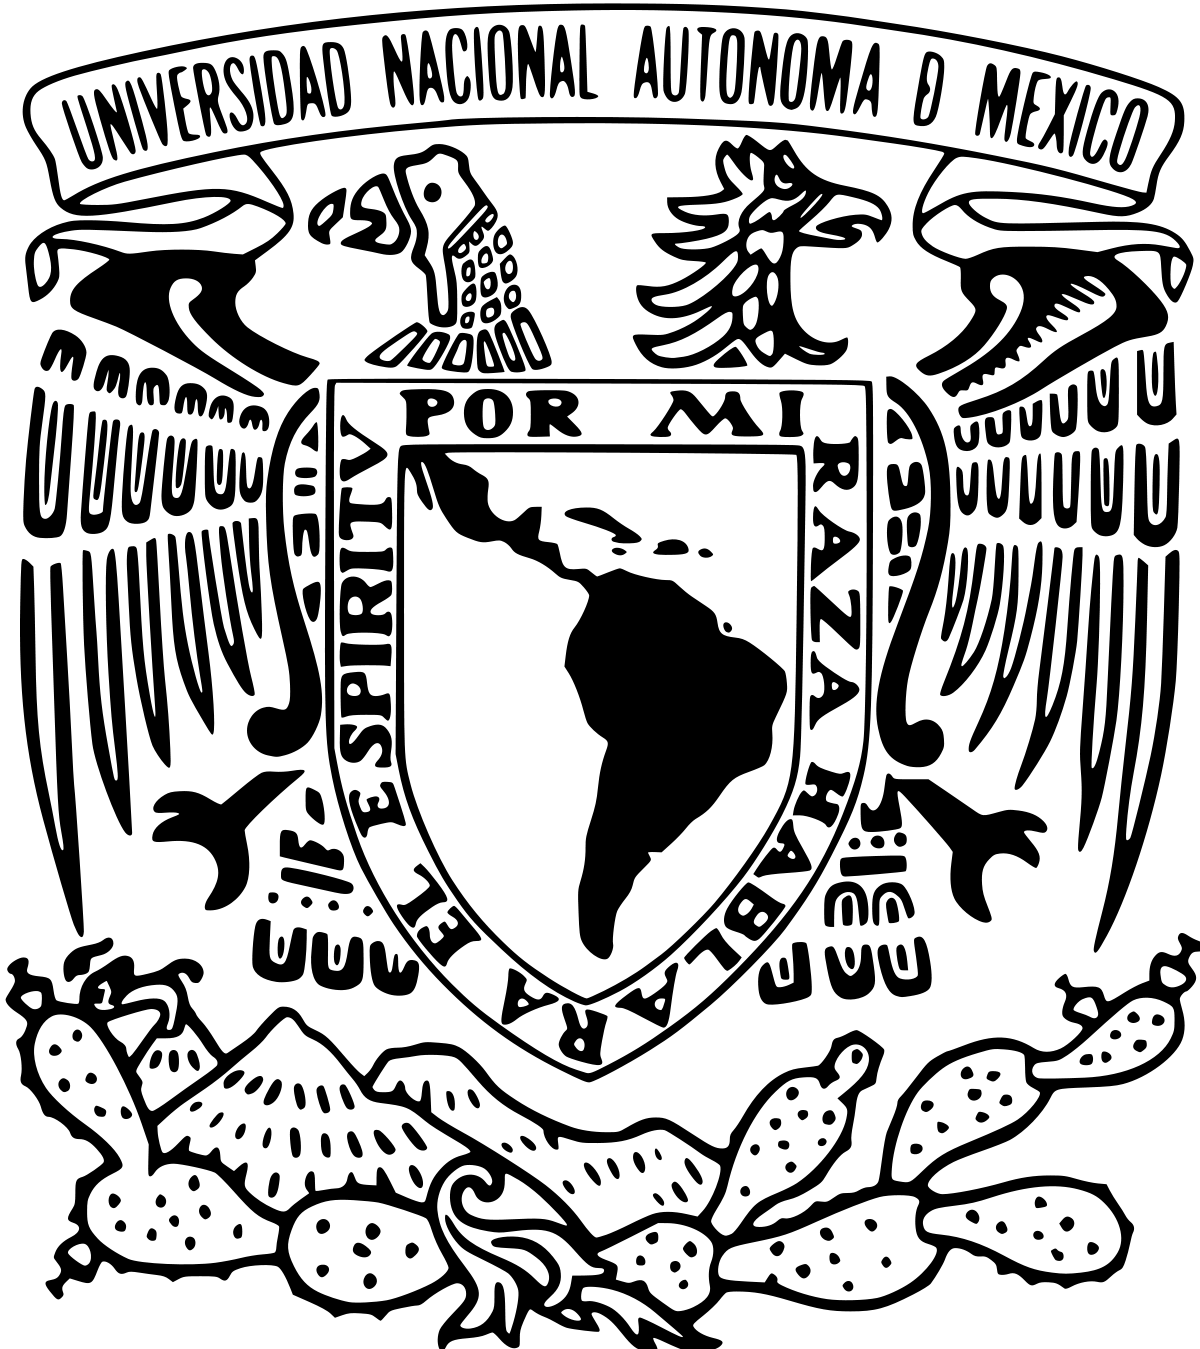
\includegraphics[height=3.2cm]{images/Logo_UNAM.png}}
         \hfill
             {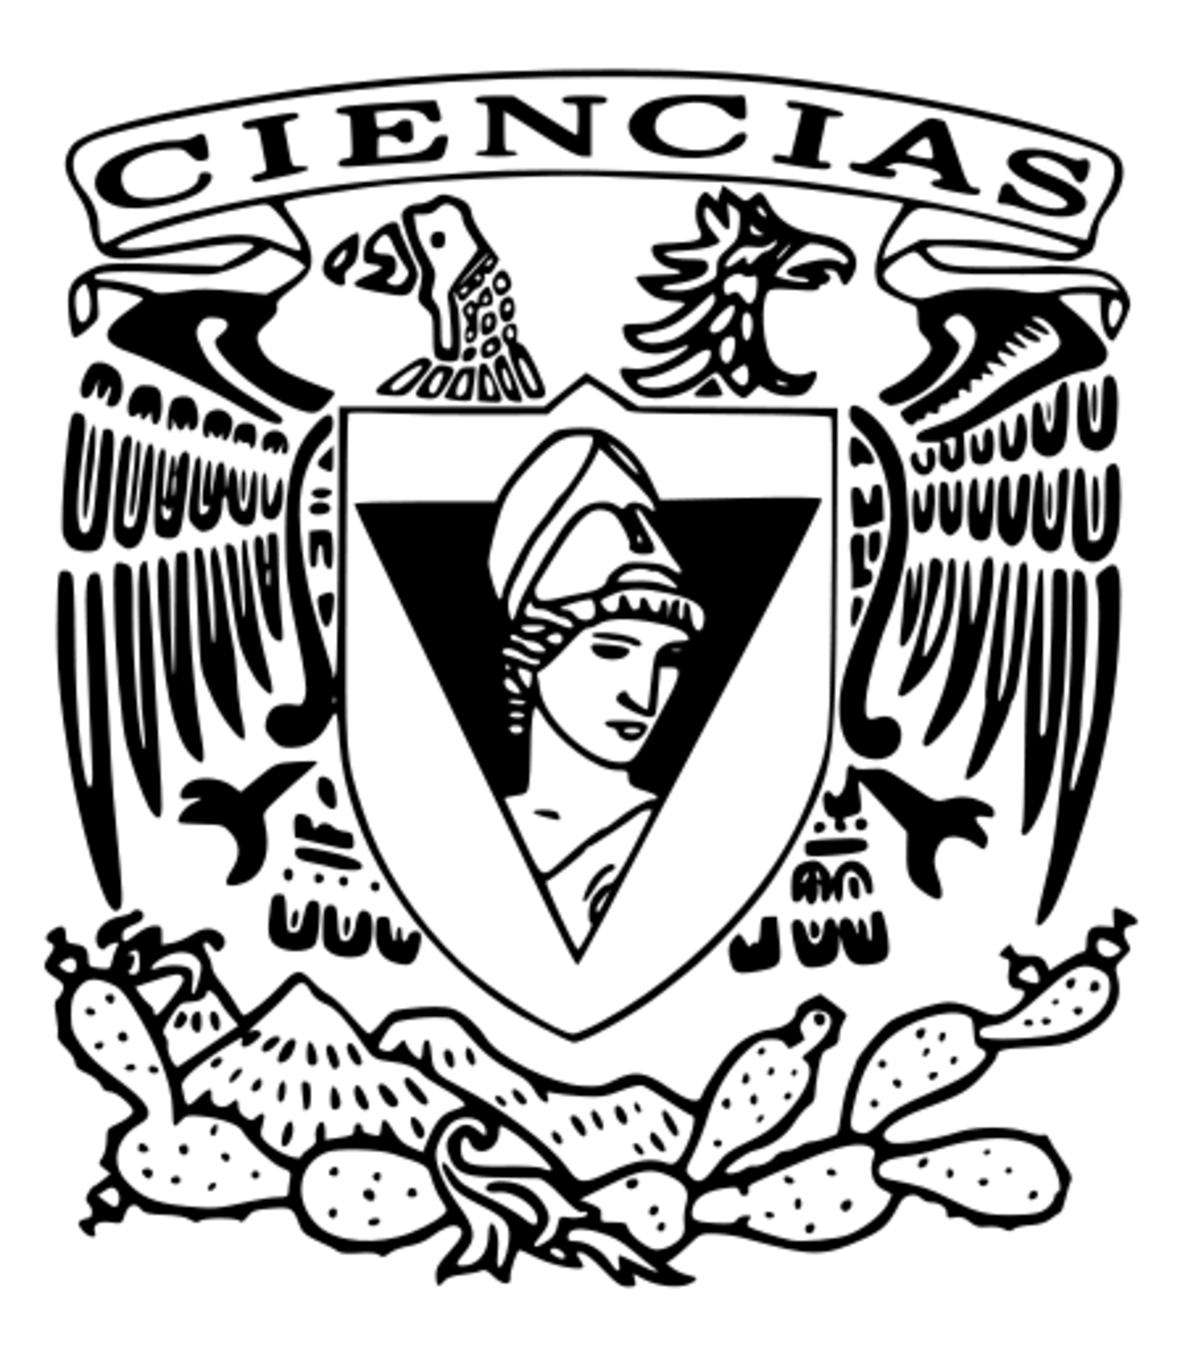
\includegraphics[height=3.2cm]{images/Logo_FC.png}\par}
             \vspace{0.5cm}
                    {\scshape\LARGE \textbf{UNIVERSIDAD NACIONAL AUTÓNOMA DE MÉXICO} \par}
                    \vspace{0.5cm}
                           {\scshape\LARGE FACULTAD DE CIENCIAS \par}
                           {\scshape\Large Ciencias de la Computación \par}
                           \vspace{0.5cm}
                                  {\scshape\Huge Compiladores \par}
                                  {\scshape\Huge Semestre 2027-1 \par}
                                  \vspace{0.8cm}
                                         {\scshape\Huge \textbf{Tarea 2} \par}
                                         {\scshape\Huge \textbf{Parsing} \par}
                                         \vspace{0.8cm}
                                                {\Large Integrantes: \par}
                                                \vspace{0.5cm}
                                                \noindent\begin{tabular}{p{10cm}p{3.5cm}}
                                                \toprule
                                                \Large
                                                Escobar Gonzalez Isaac Giovani & \Large 321336400 \\
                                                \Large
                                                Garduño Escobar Kevin Jonathan & \Large 321070629 \\
                                                \Large
                                                González Gutiérrez Antonio Tonatiuh & \Large 321195476 \\
                                                \Large
                                                Zaldivar Alanis Rodrigo & \Large 424029605 \\
                                                \bottomrule
                                                \end{tabular}\\
                                                \vspace{0.8cm}
                                                       {\itshape\Large Fecha de entrega: 00 de Noviembre de 2026 \par}
\end{titlepage}

\begin{enumerate}
    \item De las gramáticas que se muestran a continuación, reescríbelas siguiendo las indicaciones de asociación y precedencia que se indican para los operadores:
    \begin{enumerate}[label=(\alph*)]
        \item La operación :: asocia por la derecha; + y - asocian por la izquierda. El operador :: precede a + y -; + y - tienen la misma precedencia.
        \begin{verbatim}
            L := L :: L | L + element | L - element |
        \end{verbatim}
        donde element es un terminal (dado por el lexer) y la última regla refiere al elemento vacío.
        \item $>$ asocia por la derecha; ; asocia por la izquierda; ° asocia por la derecha; $\#$ no asociativo. ; precede a $>$ que precede a $\#$ que precede a °
        \begin{verbatim}
            S := S > S | S ; S | S > S | S # S | a | b
        \end{verbatim}
        Los terminales son $a$ y $b$ más los operadores indicados:
    \end{enumerate}
    \item De la siguiente gramática:
    \begin{verbatim}
        E := E + E | E - E | E * E | E / E | ( E ) | num
    \end{verbatim}
    donde \texttt{num} es terminal correspondiente a tókens numéricos (flotantes y/o enteros), realiza:
    \begin{enumerate}[label=(\alph*)]
        \item Transforma la gramática a forma normal de Chomsky.
        \item Utiliza el método de parsing CYK para parsear las cadenas: i) `2+4.5*(1+4)'; ii) `2+4.5*1+4'; y iii) `10/5-30'
    \end{enumerate}
    \item De la siguiente gramática:
    \begin{verbatim}
        S := a S b | a b | 
    \end{verbatim}
    donde $a$ y $b$ son los terminales y el último elemento corresponde a la cadena vacía $\epsilon$. Realiza:
    \begin{enumerate}[label=(\alph*)]
        \item Transforma la gramática a forma normal de Chomsky.
        \item Utiliza el método de parsing CYK para parsear las cadenas: i) `aabb'; ii) `aaaabbb'; y iii) `aaabbb'
    \end{enumerate}
    \item Dada la producción $X \rightarrow \alpha Y \beta$, demostrar que si \textsc{Null}$(\beta)$, entonces \textsc{Follow}$(X)$ $\subseteq$ \textsc{Follow}$(Y)$.
    \item Calcula las funciones \textsc{Null}, \textbf{First} y \textbf{Follow} de la siguiente gramática (considera finales a if, then, else, id y =):
    \begin{verbatim}
        S := S2 ; S | S2
        S2 := Matched | Unmatched
        Matched := if E then Matched else Matched | id = E |
        Unmatched := if E then Matched else Unmatched | if E then S2
        E := id
    \end{verbatim}
    Nótese que Matched puede derivar en la cadena vacía.
    \item Calcula \textsc{Null, First} y \textsc{Follow} de la siguiente gramática, con terminales 0, 1 y 2:
    \begin{verbatim}
        S := X S 0 |
        X := 1 X 2 | S S
    \end{verbatim}
    \item De la siguiente gramática:
    \begin{verbatim}
        S := S or T | T
        T := T and F | F
        F := not F | ( E ) | True | False
    \end{verbatim}
    \begin{enumerate}[label=(\alph*)]
        \item Elimina la recursión izquierda.
        \item Construye la tabla para parsing LL(1).
        \item Usa el parser LL(1) para parsear las siguientes expresiones: a) \textbf{\texttt{True or not False;}} b) \textbf{\texttt{False and not (True or False);}} y c) \textbf{\texttt{True or (False and (not True and False)).}}
    \end{enumerate}
    \item Construye el autómata LR(0) para la siguiente gramática:
    \begin{verbatim}
        E := E ~ E | E ** E | int
    \end{verbatim}
    Donde \texttt{int} corresponde a un entero del lexer. Utiliza las siguientes reglas de precedencia:
    \begin{itemize}
        \item ** precede a $\sim$
        \item ** asocia por la izquierda y $\sim$ por la derecha.
    \end{itemize}
    Para obtener un parsing para la cadena 10**2 $\sim$ 3
    \item Utiliza la gramática (expresiones booleanas) del ejercicio 7 para construir las tablas de \textbf{SLR, LR(1)} y \textbf{LALR} y parsear las cadenas que se indican en ese ejercicio.
    \item A partir de la siguiente gramática:
    \begin{verbatim}
        S := S S + | S S * | a
    \end{verbatim}
    Construye las tablas para el LR(1) canónico y LALR.
\end{enumerate}
\end{document}
